% Short sprint pitch: approach, frontier, sprint avenues, feedback.

\begin{frame}{Core idea: ask for one decision and distill its logits}
    \begin{columns}[T,onlytextwidth]
        \begin{column}{0.48\textwidth}
            \begin{block}{Prior work: distill rationales}
                Teacher writes a rationale and a 0--10 score.
                \medskip

                Student learns to reproduce the text (SFT), then RL.
                \medskip

                Every evaluation \textbf{generates hundreds of tokens}.
            \end{block}
        \end{column}
        \begin{column}{0.48\textwidth}
            \begin{block}{Gleipnir: distill the decision}
                Ask the teacher (Kimi K3) for a single token: \texttt{0} or \texttt{1}.
                \medskip

                The student matches the teacher's \textbf{probability} on that token
                (soft logit targets, LoRA).
                \medskip

                Every evaluation is \textbf{one prefill}; the score is a calibrated probability.
            \end{block}
        \end{column}
    \end{columns}
    \bigskip

    {\small No rationale targets and no RL. The teacher's uncertainty carries the
    information that rationales would otherwise have to carry.}
    \medskip

    {\scriptsize \href{https://arxiv.org/abs/2605.29601}{Sinha et al. (2026),
    \emph{Training Deliberative Monitors for Black-Box Scheming Detection}.}}
\end{frame}

\begin{frame}{Frontier quality at about 1/200 of the cost}
    \centering
    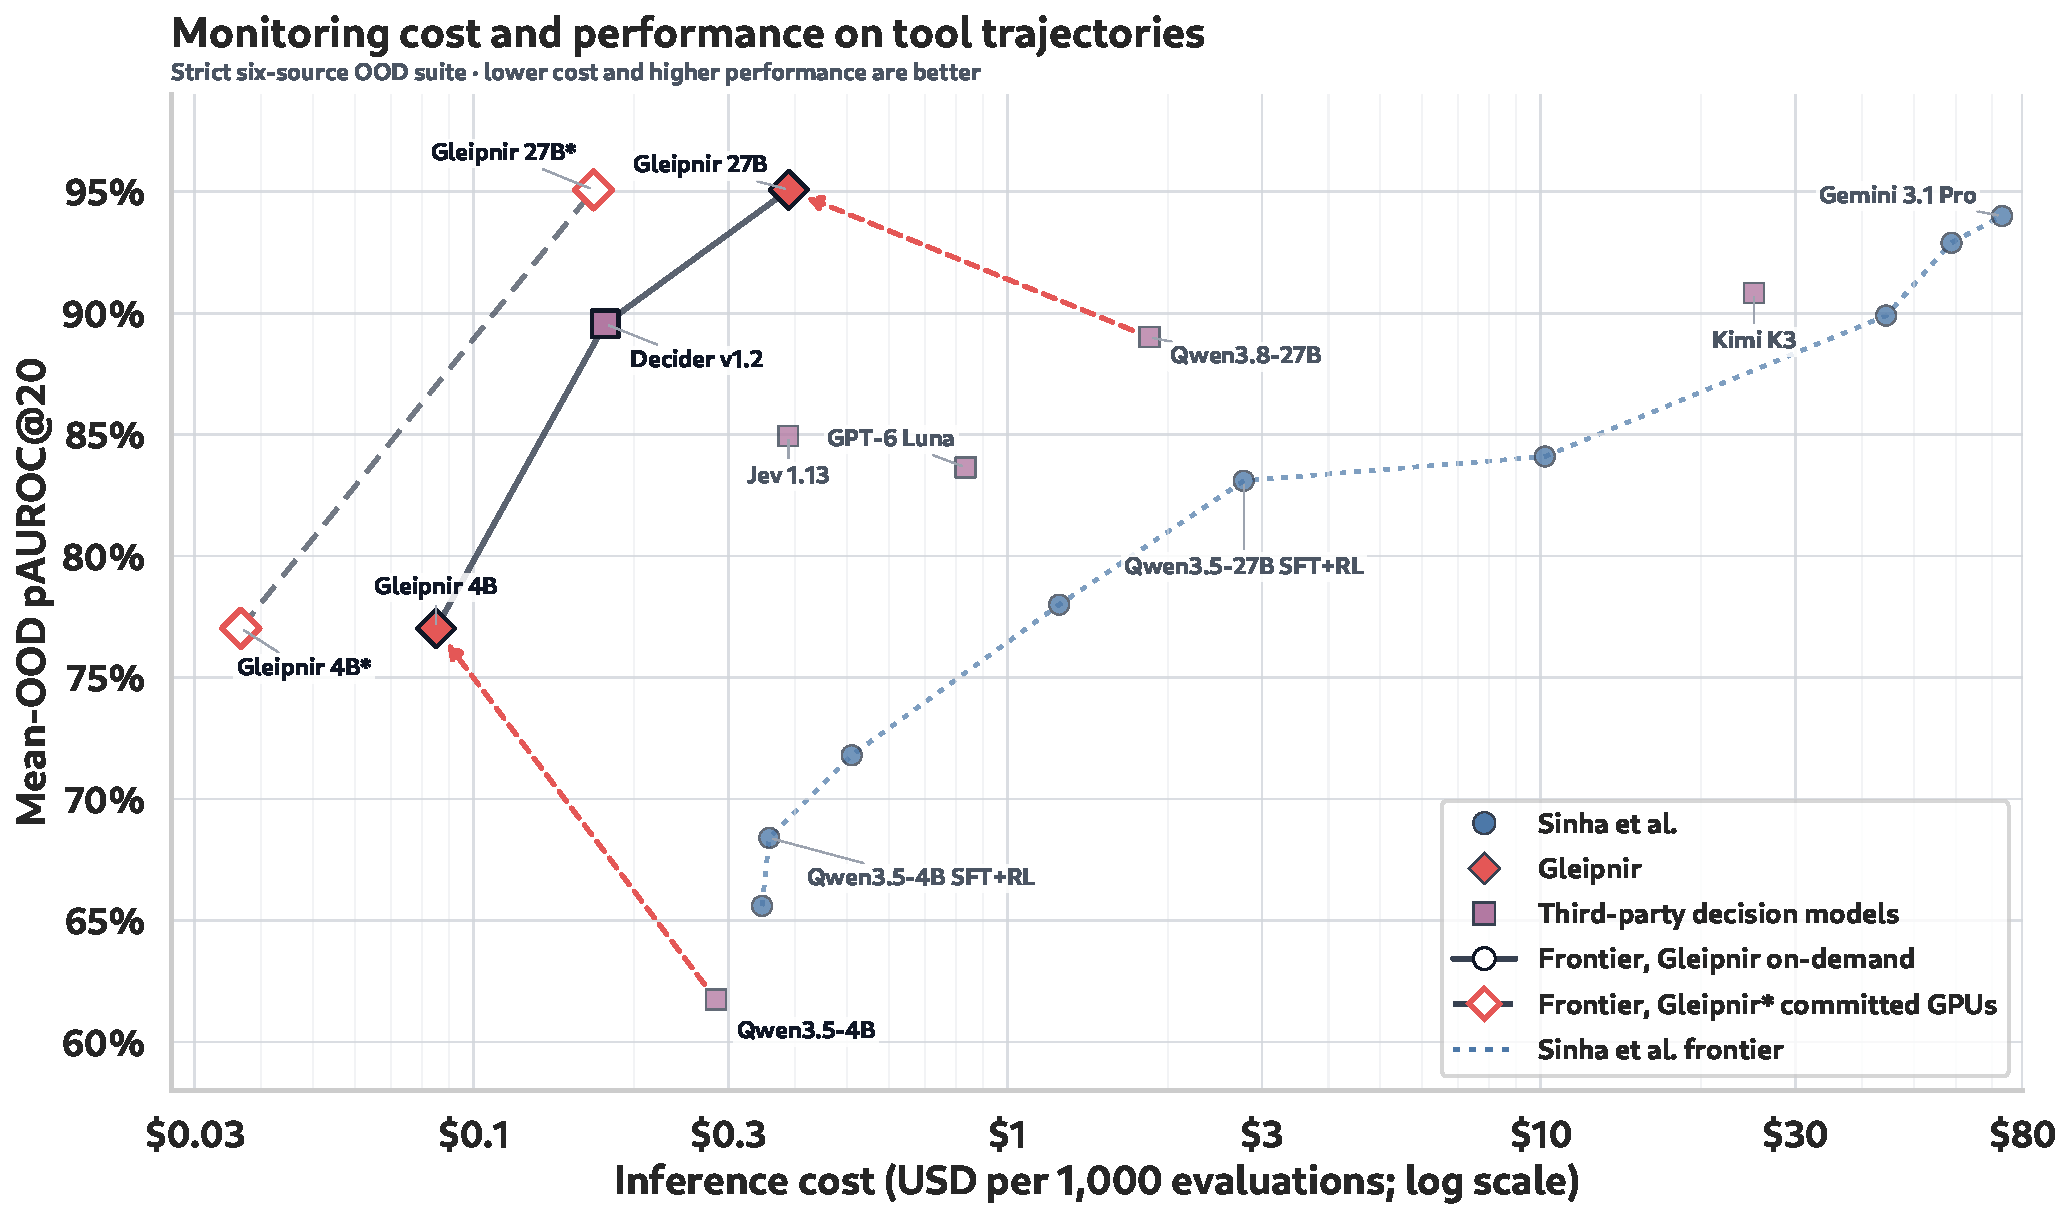
\includegraphics[height=0.80\textheight]{ood_frontier.pdf}

    {\scriptsize 6,395 OOD trajectories from six sources (Sinha et al.). Gleipnir at self-hosted B200 break-even; * committed GPUs.}
\end{frame}

\begin{frame}{Status: ahead of the proposal}
    \begin{columns}[T,onlytextwidth]
        \begin{column}{0.48\textwidth}
            \textbf{Proposal, week 1: improve the monitors}
            \begin{itemize}
                \item \alert{Done.} Gleipnir 4B (seed average + quantization-aware
                      distillation) and Gleipnir 27B are frozen release candidates.
                \item Optimized B200 serving and release packaging are built.
            \end{itemize}
        \end{column}
        \begin{column}{0.48\textwidth}
            \textbf{Proposal, week 2: stress-test them}
            \begin{itemize}
                \item \alert{Starting now}: the whole sprint goes to the second half
                      of the proposal.
                \item Both monitors are frozen, so every result describes the
                      release checkpoints.
            \end{itemize}
        \end{column}
    \end{columns}
    \bigskip

    \begin{block}{Sprint deliverable}
        A \textbf{model card} for each monitor that tells the community what it is good at,
        where it fails and how easily it can be fooled.
    \end{block}
\end{frame}

\begin{frame}{Four avenues for the model card}
    \begin{columns}[T,onlytextwidth]
        \begin{column}{0.48\textwidth}
            \begin{block}{1. Fresh benchmarks}
                \small One-shot evaluation of the frozen monitors on benchmarks never
                used in the project (MonitoringBench, SleightBench).
            \par\smallskip{\scriptsize\emph{Low effort}}
            \end{block}
            \begin{block}{2. Black-box vs.\ white-box monitors}
                \small Compare against probes. We know of no benchmark with
                \emph{open-model} agents on control tasks; building one is slow.
            \par\smallskip{\scriptsize\emph{High effort}}
            \end{block}
        \end{column}
        \begin{column}{0.48\textwidth}
            \begin{block}{3. Attacks and mechanistic fixes}
                \small The weights are public, so white-box attacks on one
                decision logit are easy to find. How easily does a decision flip?
                Can ablating directions remove unwanted traits?
            \par\smallskip{\scriptsize\emph{Medium effort}}
            \end{block}
            \begin{block}{4. Newly affordable domains}
                \small Settings that were too costly to monitor before, such as
                agent swarms: one million actions cost \$390 with Gleipnir 27B
                compared with \$73K with Gemini 3.1 Pro.
            \par\smallskip{\scriptsize\emph{Medium effort}}
            \end{block}
        \end{column}
    \end{columns}
\end{frame}

\begin{frame}{Where we would like feedback}
    \begin{itemize}
        \item \textbf{Priorities.} Which of the four avenues would make the model card most
              useful to the control community in two weeks?
        \item \textbf{Benchmarks.} Beyond MonitoringBench and SleightBench, which results would
              be most convincing?
        \item \textbf{White-box comparison.} Is there existing data with open-model agents on
              control tasks, or is building our own worth the time?
        \item \textbf{Attacks.} Which attack settings would be credible: white-box only, or
              black-box query attacks as for an API-served monitor too?
        \item \textbf{New domains.} Which setting would cheap monitoring unlock that matters
              most: swarms, long-horizon sessions, or per-token monitoring?
    \end{itemize}
\end{frame}
